% Compile from this directory with:
% pdflatex -interaction=nonstopmode bench2_alpha_report.tex

\documentclass[10pt,a4paper]{article}

\usepackage[margin=1.45cm]{geometry}
\usepackage[T1]{fontenc}
\usepackage[utf8]{inputenc}
\usepackage[table]{xcolor}
\usepackage{graphicx}
\usepackage{booktabs}
\usepackage{array}
\usepackage{parskip}
\usepackage{helvet}
\usepackage{tabularx}

\renewcommand{\familydefault}{\sfdefault}
\setlength{\parindent}{0pt}
\setlength{\parskip}{0.34em}

\definecolor{Accent}{HTML}{D56C45}
\definecolor{Ink}{HTML}{2F2924}
\definecolor{Panel}{HTML}{F7F4EE}
\definecolor{Rule}{HTML}{A89D8B}

\graphicspath{{./}}

\begin{document}
\color{Ink}

\begin{center}
    {\LARGE\bfseries Keepalive Benchmark Report}\\[0.20em]
    {\large Alpha 0 and Alpha 100 Comparison}\\[0.45em]
    {\color{Accent}\rule{0.92\linewidth}{1.2pt}}
\end{center}

\begin{table}[h]
\centering
\small
\renewcommand{\arraystretch}{1.12}
\rowcolors{2}{Panel}{white}
\begin{tabularx}{\linewidth}{>{\bfseries\raggedright\arraybackslash}p{0.28\linewidth} X}
Target host & 192.168.2.2 \\
Compared paths & Vanilla keepalive path through the TLS proxy on port 8444 versus sendfd prototype gateway on port 9444 \\
Prototype faasd patch & OpenFaaS gateway patched to load \texttt{bench2gw}, expose a second TLS listener on \texttt{:9444}, and move live TCP file descriptors plus exported TLS state through Unix sockets in \texttt{/run/bench2} \\
Functions & \texttt{bench2-fn-a} and \texttt{bench2-fn-b} \\
Payload sizes & 64 B, 256 B, 1 KiB, 4 KiB, 16 KiB, 64 KiB, 128 KiB, 256 KiB, 512 KiB, 1 MiB \\
Measured requests & 100 recorded requests per payload size, hence 1000 recorded requests per mode and per alpha \\
Warmup & 20 warmup requests per payload size, not included in the CSV files or in the figures \\
TLS reuse & \texttt{requests\_per\_conn = 50} for both vanilla and prototype \\
Alpha = 0 & strict alternation between the two container functions \\
Alpha = 100 & all requests pinned to the same function container, with \texttt{bench2-fn-a} used as the owner \\
Metric shown & mean time as bars and p99 time as dashed curves, in milliseconds \\
Axis scale & logarithmic y-axis, but tick labels remain written as plain time values \\
\end{tabularx}
\end{table}

{\small
\noindent\fcolorbox{Rule}{Panel}{%
\parbox{\dimexpr\linewidth-2\fboxsep-2\fboxrule\relax}{%
\textbf{What is measured.}
Each plotted sample is the ingress-to-owner-read time of one request, reported as \texttt{delta\_ns = top2 - top1}. Both timestamps are taken from the same Arm architectural counter. In the vanilla path, \texttt{top1} is stamped in the TLS proxy on port 8444 after \texttt{bench2\_wait\_readable()} confirms that encrypted bytes are already present in the kernel receive buffer, and immediately before \texttt{wolfSSL\_read()} and forwarding to the local OpenFaaS gateway. \texttt{top2} is stamped in the final owner container after the full HTTP request body has been read.

In the prototype, there are two \texttt{top1} cases. For the first request on a connection, the sendfd gateway on port 9444 waits for readable bytes, stamps \texttt{top1}, then executes \texttt{tls\_read\_peek()} and exports the wolfSSL session state; the raw TCP fd, the exported TLS state and the stamped \texttt{top1} are then dispatched to the selected container. For a later keepalive request that first arrives in the wrong container, that wrong-owner worker itself waits for readability, stamps \texttt{top1} immediately before its own \texttt{tls\_read\_peek()}, detects that the request targets the other function, exports the live TLS state, and sends the raw fd plus the already-stamped payload back to the gateway over the relay socket. The gateway redispatches the same fd and payload to the correct owner without restamping \texttt{top1}. Therefore, in the relay case, the reported time includes the wrong-owner peek, the hand-back to the gateway, the redispatch, and the final owner read up to full request-body completion. Response generation and the response path back to the client are excluded.}}

\textbf{What we patched in faasd.}
The prototype does not use stock faasd as-is. We patched the OpenFaaS gateway build so that \texttt{gateway/main.go} imports and starts a new Go/CGO package named \texttt{bench2gw} when \texttt{BENCH2GW\_ENABLE=1}. This package adds the extra TLS listener on port 9444, performs the TLS peek and wolfSSL export through \texttt{libtlspeek}, and dispatches or relays live TCP file descriptors plus serialized TLS state through per-function Unix sockets under \texttt{/run/bench2} and the relay socket \texttt{/run/bench2/relay.sock}. The vanilla path does not use these gateway modifications; it keeps the normal local OpenFaaS HTTP gateway on port 8080 and relies on the separate TLS proxy on port 8444.

\textbf{Timing instrumentation.}
No external profiler was used to obtain the plotted request times. The timing tool is the in-code helper \texttt{bench2\_rdtsc()} with \texttt{bench2\_cntfrq()} from \texttt{bench2\_rdtsc.h}. On the Raspberry Pi arm64 platform, these helpers read the architectural virtual counter \texttt{CNTVCT\_EL0} and its frequency register \texttt{CNTFRQ\_EL0}. The helper \texttt{bench2\_wait\_readable()} uses \texttt{ioctl(FIONREAD)} and a yield loop so that \texttt{top1} is taken only once request bytes are already present in the kernel receive buffer. The C components emit \texttt{delta\_cycles} and \texttt{cntfrq}, and the Python sweep script converts them into \texttt{delta\_ns}, which is then plotted in milliseconds.

\textbf{How to read the figures.}
For each payload size, the filled bars show the mean time and the dashed curves show the p99 time over the 100 recorded requests. Lower values are better. The two figures isolate the two locality extremes: in Figure~1 every request alternates between the two functions, while in Figure~2 all requests stay on the same function container.

\textbf{Interpretation.}
Under \(\alpha = 0\), the prototype stays below the vanilla path for every payload size on both statistics. At 64 B, the prototype reduces the mean time from 31.24 ms to 0.83 ms and the p99 from 54.26 ms to 1.58 ms. At 1 MiB, the prototype still keeps a clear advantage, with 100.31 ms versus 587.62 ms on the mean and 312.17 ms versus 855.13 ms on the p99. Across the ten payload points, the vanilla-to-prototype ratio averages about 21.8x on the mean and 20.2x on the p99.

Under \(\alpha = 100\), the gap becomes even larger for small and medium payloads. At 64 B, the prototype reaches 0.15 ms mean and 0.87 ms p99, whereas the vanilla path remains at 53.66 ms mean and 125.33 ms p99. Even at 1 MiB, the prototype still measures 104.15 ms mean and 314.42 ms p99, compared with 1498.30 ms mean and 2179.40 ms p99 for vanilla. Across the ten payload points, the vanilla-to-prototype ratio averages about 115.5x on the mean and 66.0x on the p99. The locality effect is also different in the two architectures: moving from \(\alpha = 0\) to \(\alpha = 100\) improves the prototype on small payloads and leaves it almost unchanged on the largest ones, while the vanilla path becomes slower overall. This indicates that the prototype benefits from keeping ownership in the same container, whereas the dominant overhead in the vanilla path remains the forwarding chain itself.
}

\newpage

\begin{center}
    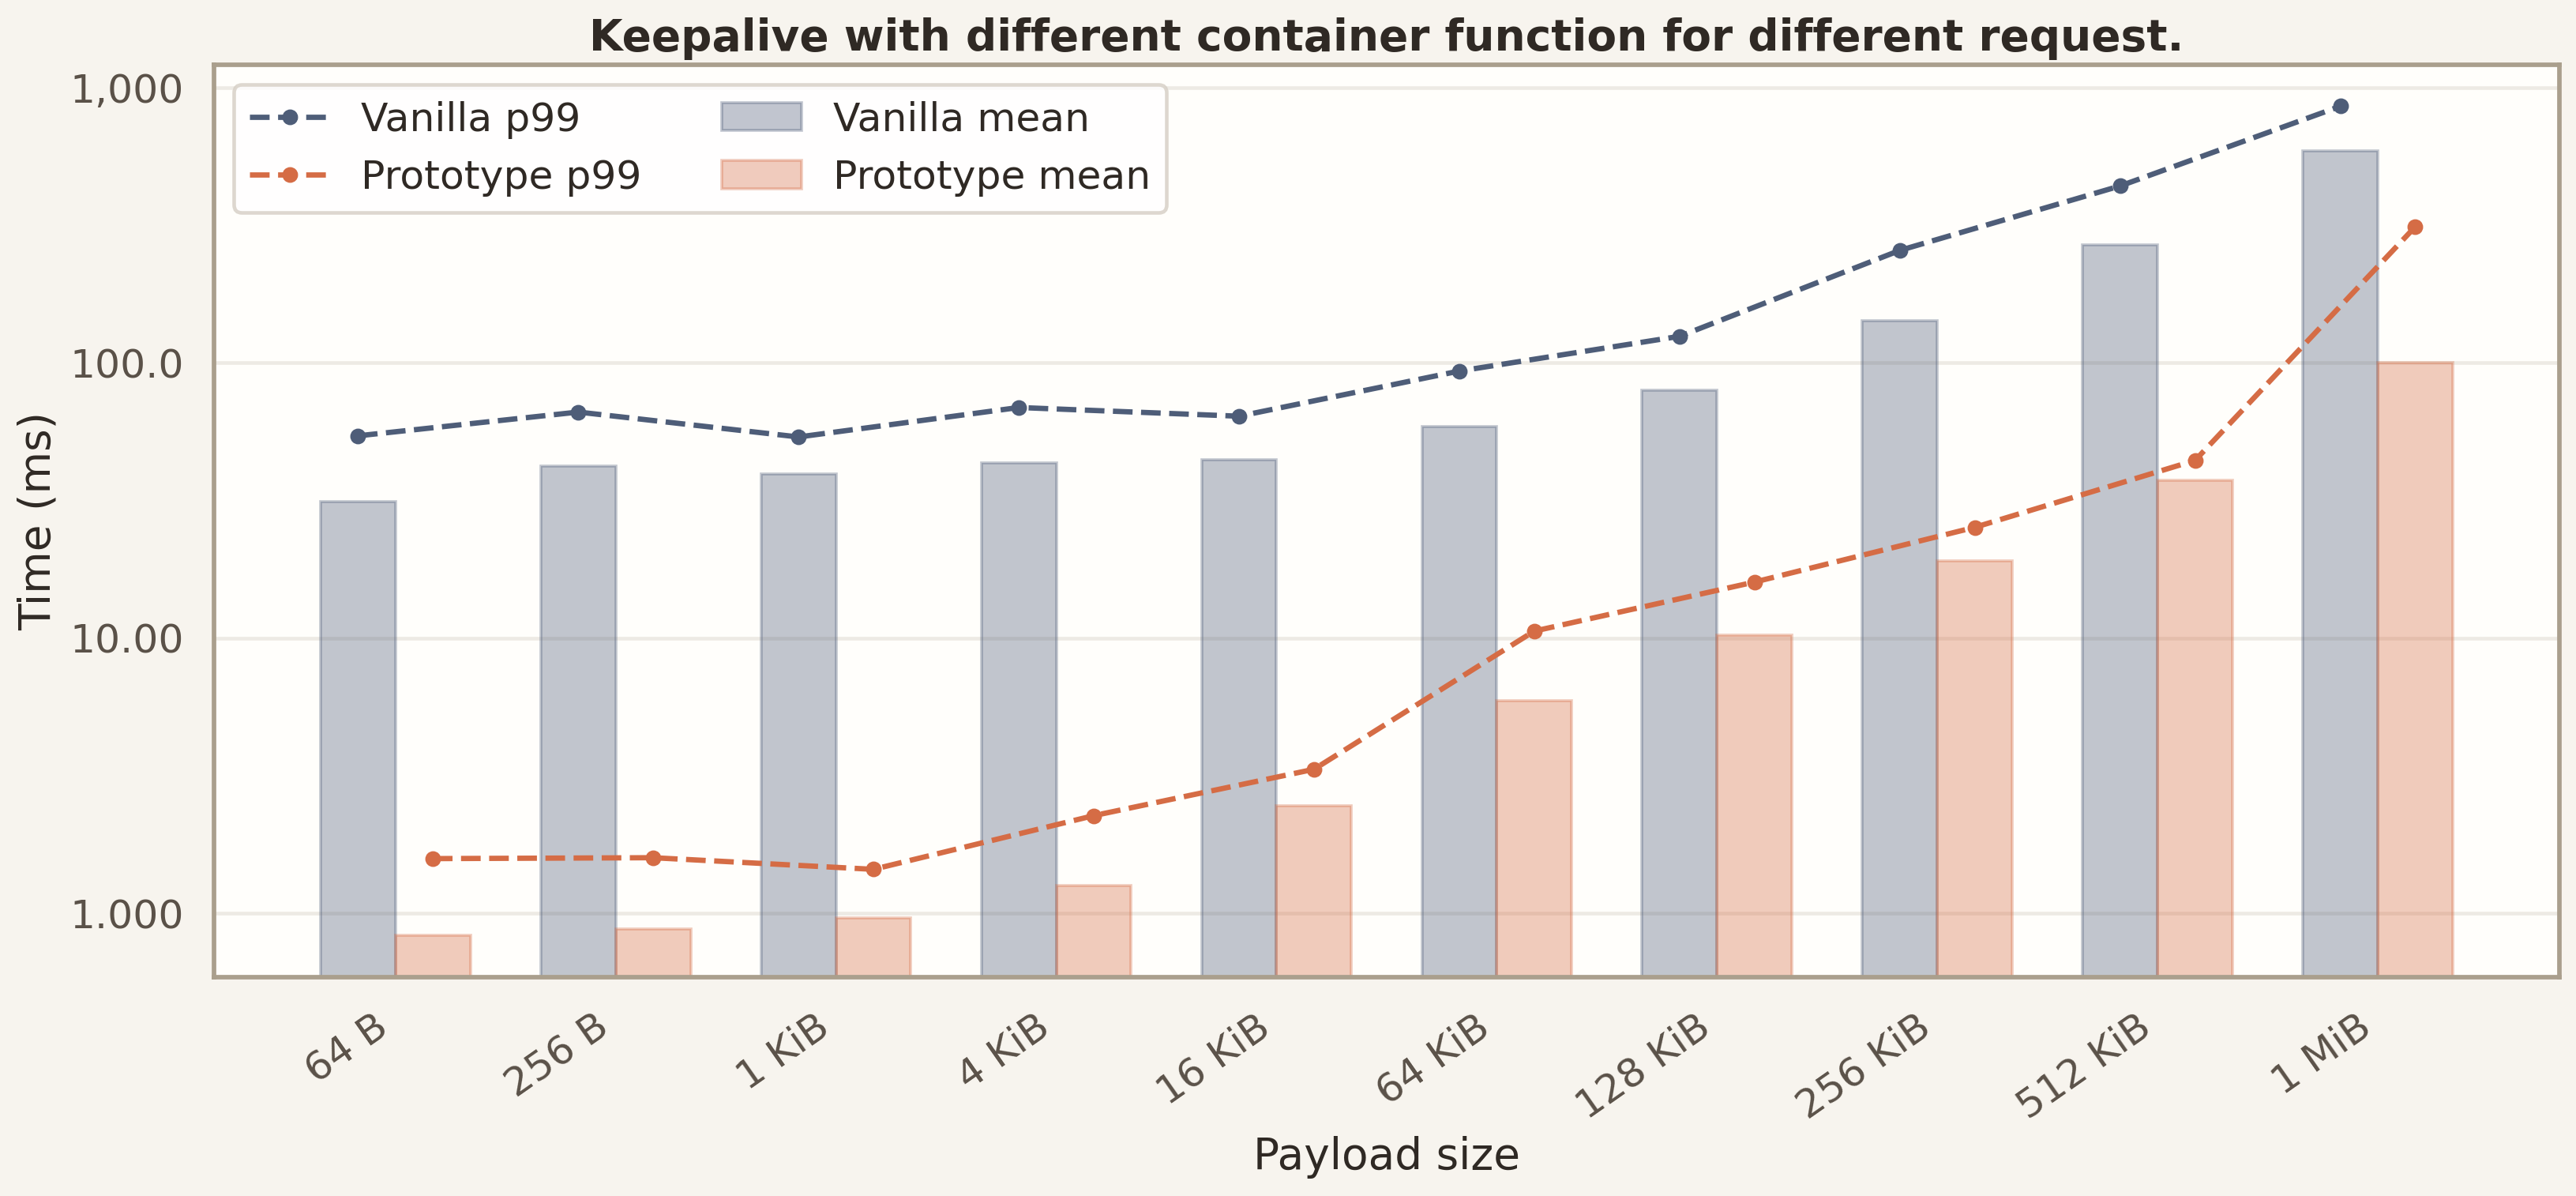
\includegraphics[width=0.94\linewidth]{bench2_alpha0_mean_p99.png}\\[0.30em]
    {\small\textbf{Figure 1.} Keepalive with different container function for different request.}

    \vspace{0.85em}

    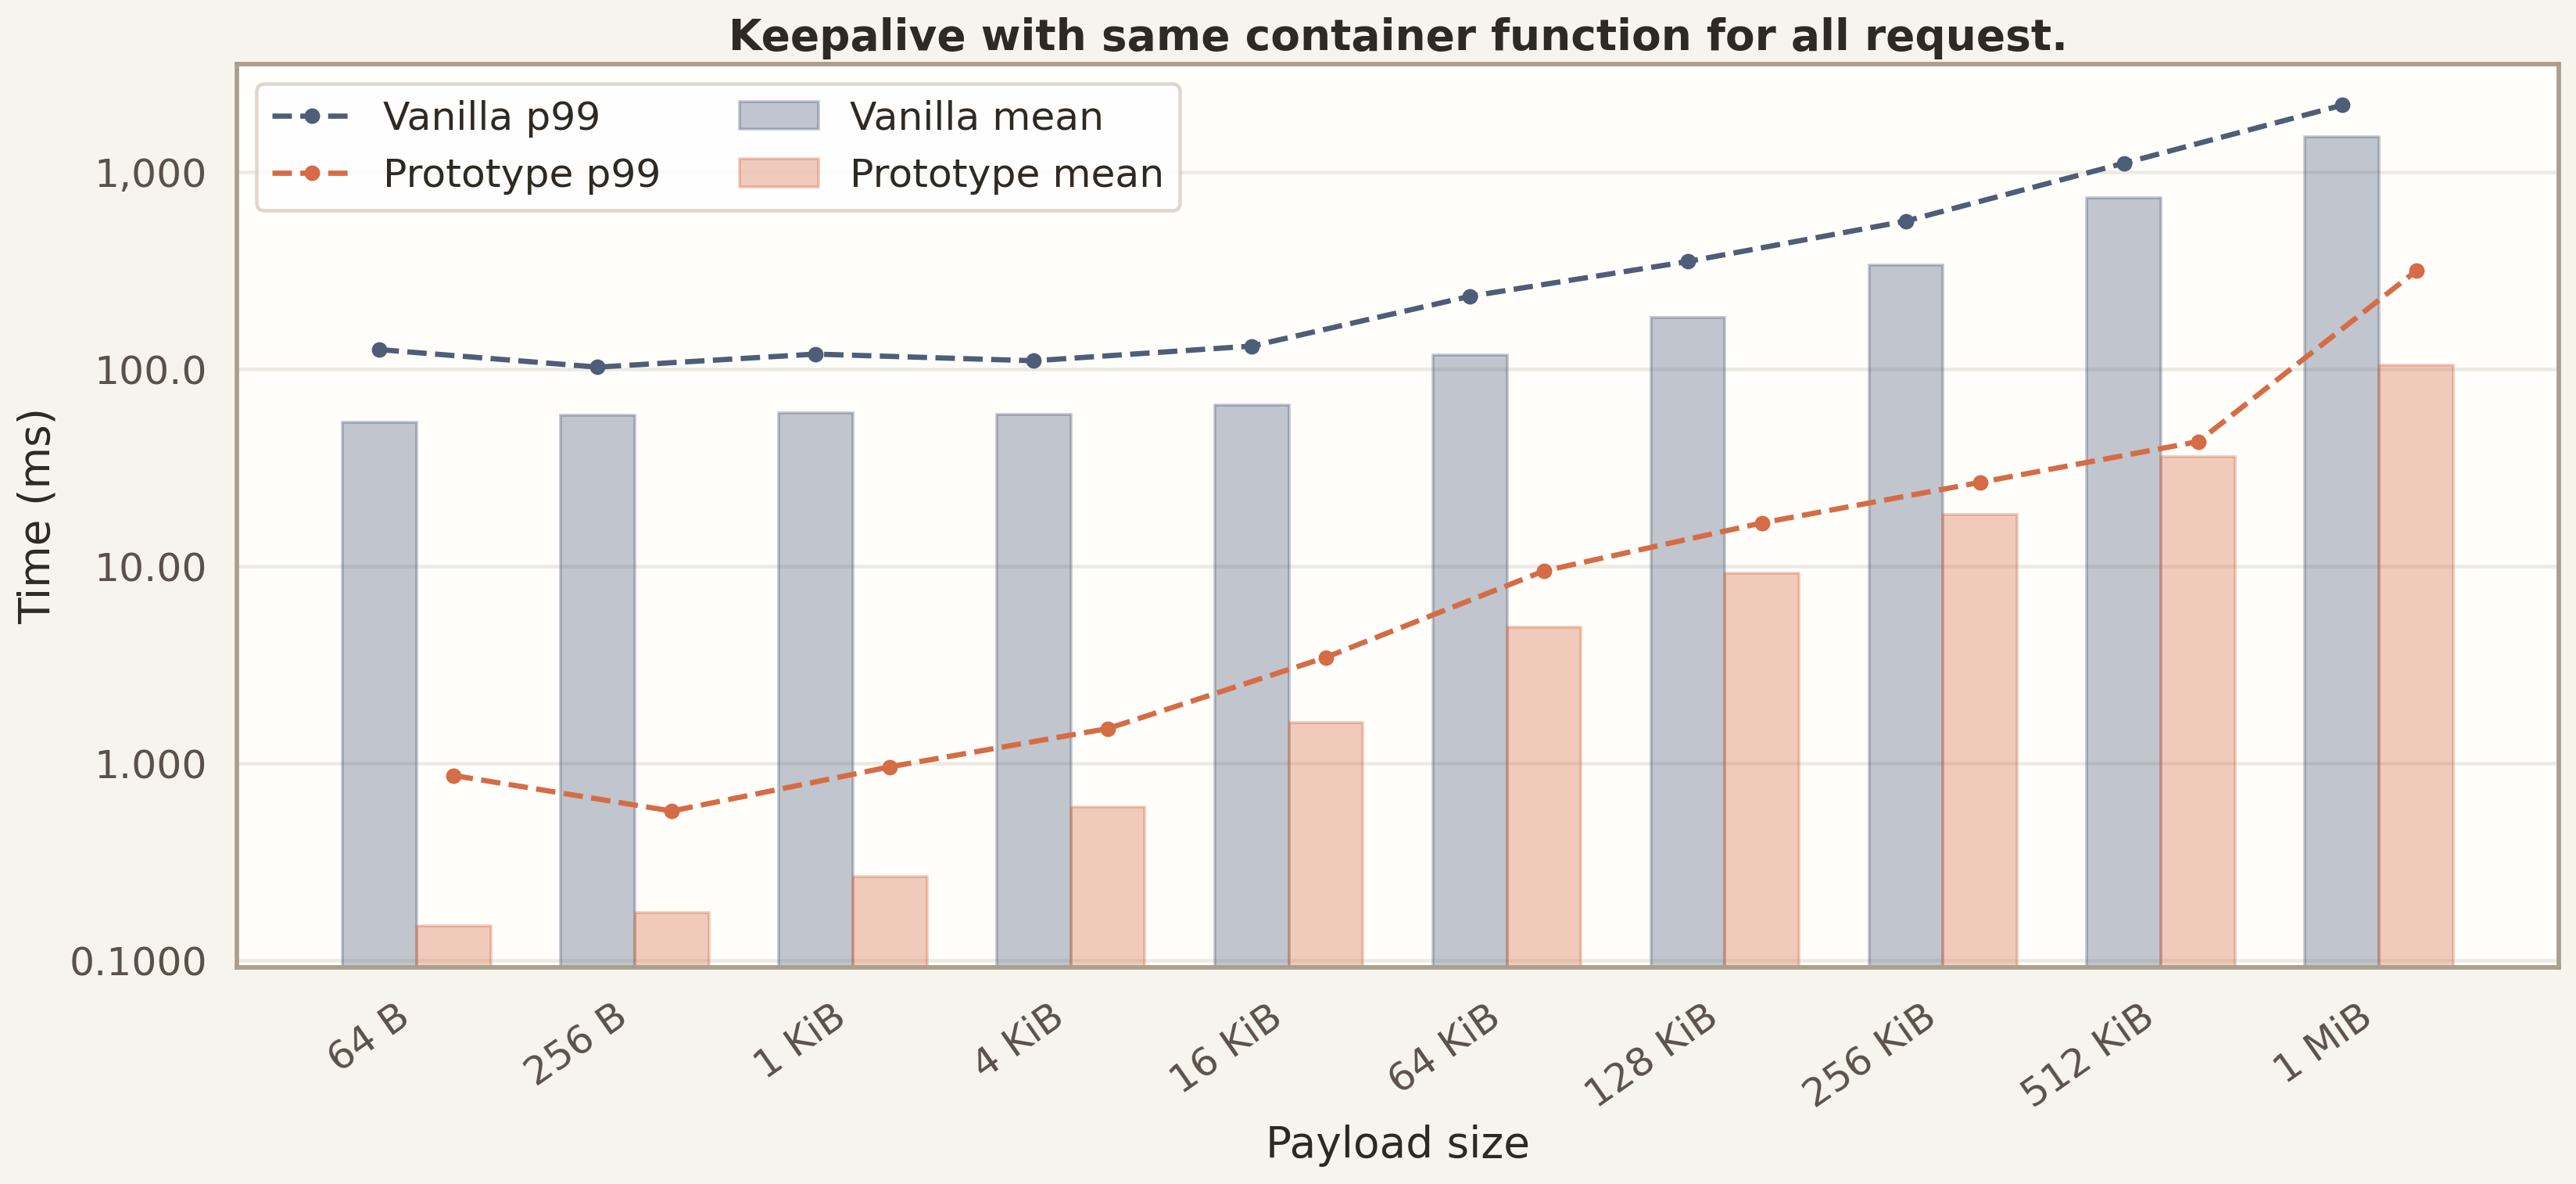
\includegraphics[width=0.94\linewidth]{bench2_alpha100_mean_p99.png}\\[0.30em]
    {\small\textbf{Figure 2.} Keepalive with same container function for all request.}
\end{center}

\end{document}
